\documentclass[11pt]{article}

\usepackage[letterpaper,margin=0.8in]{geometry}
\usepackage[T1]{fontenc}
\usepackage[utf8]{inputenc}
\usepackage{lmodern}
\usepackage{graphicx}
\usepackage{booktabs}
\usepackage{tabularx}
\usepackage{array}
\usepackage{xcolor}
\usepackage{enumitem}
\usepackage{hyperref}
\usepackage{listings}
\usepackage{fancyhdr}

\graphicspath{{../../assets/}{../../assets/figures/}{assets/}{assets/figures/}}

\definecolor{accent}{HTML}{376D63}
\definecolor{lightbox}{HTML}{F4F8F6}
\definecolor{rulegray}{HTML}{C9C9C9}

\hypersetup{
  colorlinks=true,
  linkcolor=accent,
  urlcolor=accent,
  citecolor=accent
}

\setlength{\parindent}{0pt}
\setlength{\parskip}{0.55em}
\setlist[itemize]{leftmargin=1.4em,itemsep=0.2em,topsep=0.2em}

\pagestyle{fancy}
\fancyhf{}
\lfoot{\footnotesize RoboCerebra future plan - subtask-level failure detection}
\rfoot{\footnotesize Page \thepage}
\renewcommand{\headrulewidth}{0pt}
\renewcommand{\footrulewidth}{0.4pt}

\newcolumntype{Y}{>{\raggedright\arraybackslash}X}
\newcommand{\code}[1]{\texttt{\detokenize{#1}}}

\lstdefinestyle{pseudo}{
  basicstyle=\ttfamily\small,
  backgroundcolor=\color{gray!8},
  frame=single,
  rulecolor=\color{rulegray},
  framerule=0.4pt,
  xleftmargin=0.4em,
  xrightmargin=0.4em,
  breaklines=true,
  columns=fullflexible
}

\newenvironment{summarybox}
{\begin{center}\setlength{\fboxsep}{8pt}\fcolorbox{rulegray}{lightbox}\bgroup\begin{minipage}{0.88\linewidth}}
{\end{minipage}\egroup\end{center}}

\title{\textbf{RoboCerebra Future Plan: Subtask-Level Failure Detection and Recovery}}
\author{Felix Doublet}
\date{}

\begin{document}
\maketitle

\textit{Prepared as a short technical note on how the RoboCerebra benchmark can be used to identify the failed subtask in a long-horizon rollout, then restart from the previous GT subtask boundary or ask the robot to return to the GT pose.}

\begin{summarybox}
\textbf{Executive summary.}
RoboCerebra is useful not only because it reports whole-episode success, but because its evaluation structure can expose where a long-horizon execution first fails. Each task is decomposed into ordered step descriptions, each step can be linked to a demonstration boundary state, and the goal predicates in \code{goal.json} can be assigned to task steps. Therefore, if the predicate expected at subtask $k$ does not become true within the step-$k$ horizon, or if a predicate completed before $k$ regresses, the benchmark can label subtask $k$ as the failure point.
\end{summarybox}

\section{Benchmark Structure Used for Diagnosis}

The evaluator already contains the pieces needed for subtask-level diagnosis. The file \code{task_description.txt} defines the ordered subtask instructions and their demonstration frame ranges. The evaluator loads those start indices from the demonstration states in \code{demo.hdf5}. In parallel, \code{goal.json} stores object-state relations, and the newer format includes a \code{task_step} annotation. This makes it possible to map each success predicate to the subtask that is supposed to achieve it.

The important point is that a rollout does not need to be judged only at the final timestep. At each step boundary, the evaluator can call \code{env._check_success(goal)} and compare the number and identity of completed predicates against the expected predicates for the current subtask. This turns a single whole-task failure into a structured diagnosis: completed prefix, first failing subtask, missing predicate, and any regression of earlier progress.

\begin{figure}[htbp]
  \centering
  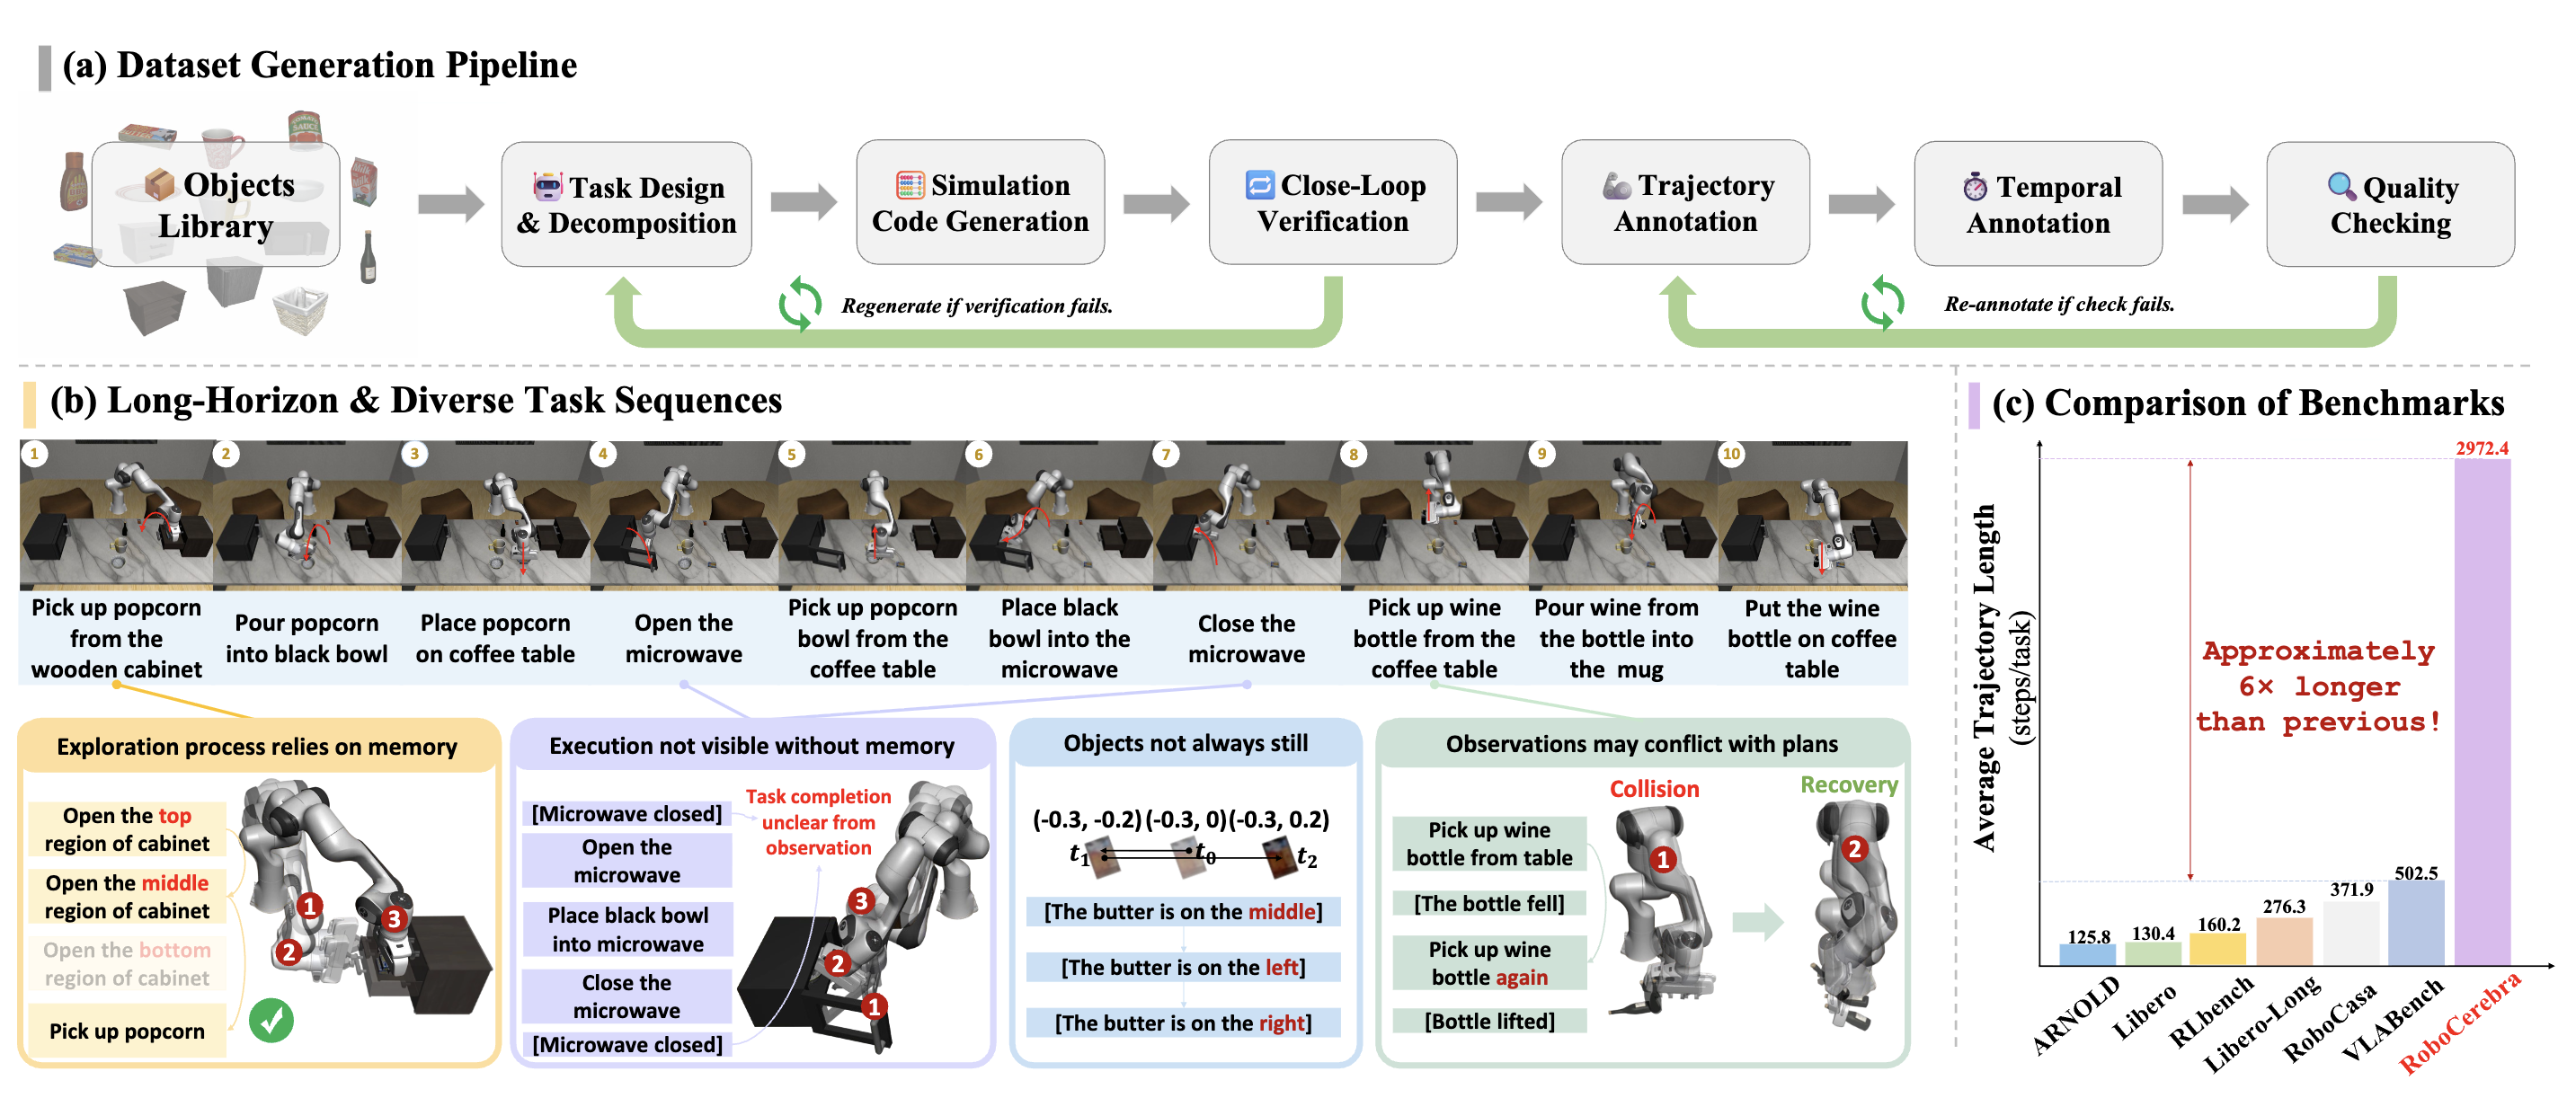
\includegraphics[width=0.92\linewidth]{overview.png}
  \caption{RoboCerebra decomposes long-horizon robot tasks into step sequences; this structure is the basis for subtask-level diagnosis.}
\end{figure}

\section{Detecting the Failed Subtask}

For subtask $k$, I will define success as the transition from the predicate set before $k$ to the predicate set expected after $k$, while maintaining all predicates that were completed before $k$. A failure is assigned to $k$ when the expected predicate does not change, changes in the wrong direction, or takes longer than the step horizon. The same measurement can be used in the Ideal, Random\_Disturbance, Observation\_Mismatching, and Mix settings.

\begin{table}[htbp]
\centering
\caption{Signals for subtask-level failure detection.}
\begin{tabularx}{\linewidth}{>{\raggedright\arraybackslash}p{0.22\linewidth}Y Y}
\toprule
\textbf{Signal} & \textbf{Computation} & \textbf{Failure interpretation} \\
\midrule
Predicate progress & Compare \code{env._check_success(goal)} before and after subtask $k$. & The expected predicate for subtask $k$ is still false. \\
Regression & Check whether predicates completed before $k$ become false after policy actions. & The policy damaged previous progress. \\
Time budget & Use the fixed segment horizon controlled by \code{switch_steps}. & The policy timed out at subtask $k$. \\
State deviation & Compare the current object and robot pose against the GT boundary state. & The rollout has moved off the demonstrated state manifold. \\
Perturbation response & Evaluate the same logic under Random\_Disturbance, Observation\_Mismatching, and Mix. & The model is not robust to controlled disturbance. \\
\bottomrule
\end{tabularx}
\end{table}

The monitor can be implemented with the following step-boundary loop:

\begin{lstlisting}[style=pseudo]
for subtask k:
    progress_before = check_success(goal)
    run policy for the step-k horizon
    progress_after = check_success(goal)
    if expected_predicates[k] are not completed:
        label failure at k
    if previous_predicates regressed:
        label recovery-required regression
    log missing predicates, pose deviation, video clip, and recovery mode
\end{lstlisting}

This produces a more useful dataset than final success alone. A failed episode can still contribute the completed prefix, the exact first failure location, and a controlled starting state for recovery experiments.

\section{Recovery Protocols After Failure}

After identifying the failing subtask, I propose evaluating two recovery protocols. They should be reported separately because they answer different questions: one is a clean diagnostic reset, and the other is a physically meaningful recovery attempt.

\begin{table}[htbp]
\centering
\caption{Recovery protocols after detecting subtask failure.}
\begin{tabularx}{\linewidth}{>{\raggedright\arraybackslash}p{0.24\linewidth}Y Y}
\toprule
\textbf{Recovery mode} & \textbf{Procedure} & \textbf{What it tests} \\
\midrule
A. GT-state restart & Set the simulator to the saved demonstration state at the boundary after subtask $k-1$. Reset the policy queue/state, mark prior predicates complete with the resume handler, and restart from the step-$k$ instruction. & Clean per-subtask competence when previous progress is guaranteed correct. \\
B. Robot-to-GT-pose recovery & Command the robot back to the GT EEF or joint pose at the previous boundary. Recheck prior predicates and continue from subtask $k$; use full GT-state restart only if the world is invalid. & Embodied recoverability under a more realistic robot protocol. \\
\bottomrule
\end{tabularx}
\end{table}

The GT-state restart should be treated as the controlled upper-bound condition. In the current evaluator, it corresponds to setting the simulator to the saved step state and using the resume handler to mark all prior subtasks as logically complete. This isolates whether the model can solve subtask $k$ when the previous subtasks are correct.

The robot-to-GT-pose condition is closer to the real robot setting. Instead of teleporting the entire simulator state, the robot is asked to move back to the GT end-effector or joint pose at the previous boundary. Prior predicates are then checked again. If the world is still valid, the policy resumes from the failing subtask; if the world is invalid, the evaluator can fall back to GT-state restart and record that the physical recovery failed.

\section{Experiment Plan}

The next implementation step is to add a per-subtask attempt record to the evaluator output.

\begin{itemize}
  \item For each subtask, store the start state index, instruction text, expected predicates, completed predicates, missing predicates, segment video path, and failure type.
  \item Run three conditions: normal chained rollout, isolated subtask rollout from the GT previous boundary, and recovery rollout after a detected failure.
  \item Compare task regimes: Ideal, Random\_Disturbance, Observation\_Mismatching, Mix, Memory\_Execution, and Memory\_Exploration.
  \item Report first-failing-subtask distribution, per-subtask isolated success, GT-state-restart recovery, robot-to-GT-pose recovery, and the chained-vs-isolated gap.
\end{itemize}

The resulting analysis should show whether the model's main limitation is high-level planning, low-level execution, memory over a long horizon, or inability to recover after the world state drifts away from the demonstration distribution.

\section{Current Evidence}

The local checkpoint summaries already track subtask completion independently from episode success. This is evidence that the current infrastructure can measure partial progress and can be extended into a more explicit subtask-failure diagnostic benchmark.

\begin{table}[htbp]
\centering
\caption{Checkpoint-summary values used in the current document.}
\begin{tabularx}{\linewidth}{>{\raggedright\arraybackslash}p{0.16\linewidth}Y Y Y}
\toprule
\textbf{Model} & \textbf{Step-0 subtask} & \textbf{Best checkpoint} & \textbf{Latest checkpoint in CSV} \\
\midrule
PI0 & 16.6\% & 19.9\% at 25,000 steps & 18.1\% at 125,000 steps \\
PI0.5 & 14.4\% & 19.6\% at 35,000 steps & 17.9\% at 100,000 steps \\
\bottomrule
\end{tabularx}
\end{table}

\begin{figure}[htbp]
  \centering
  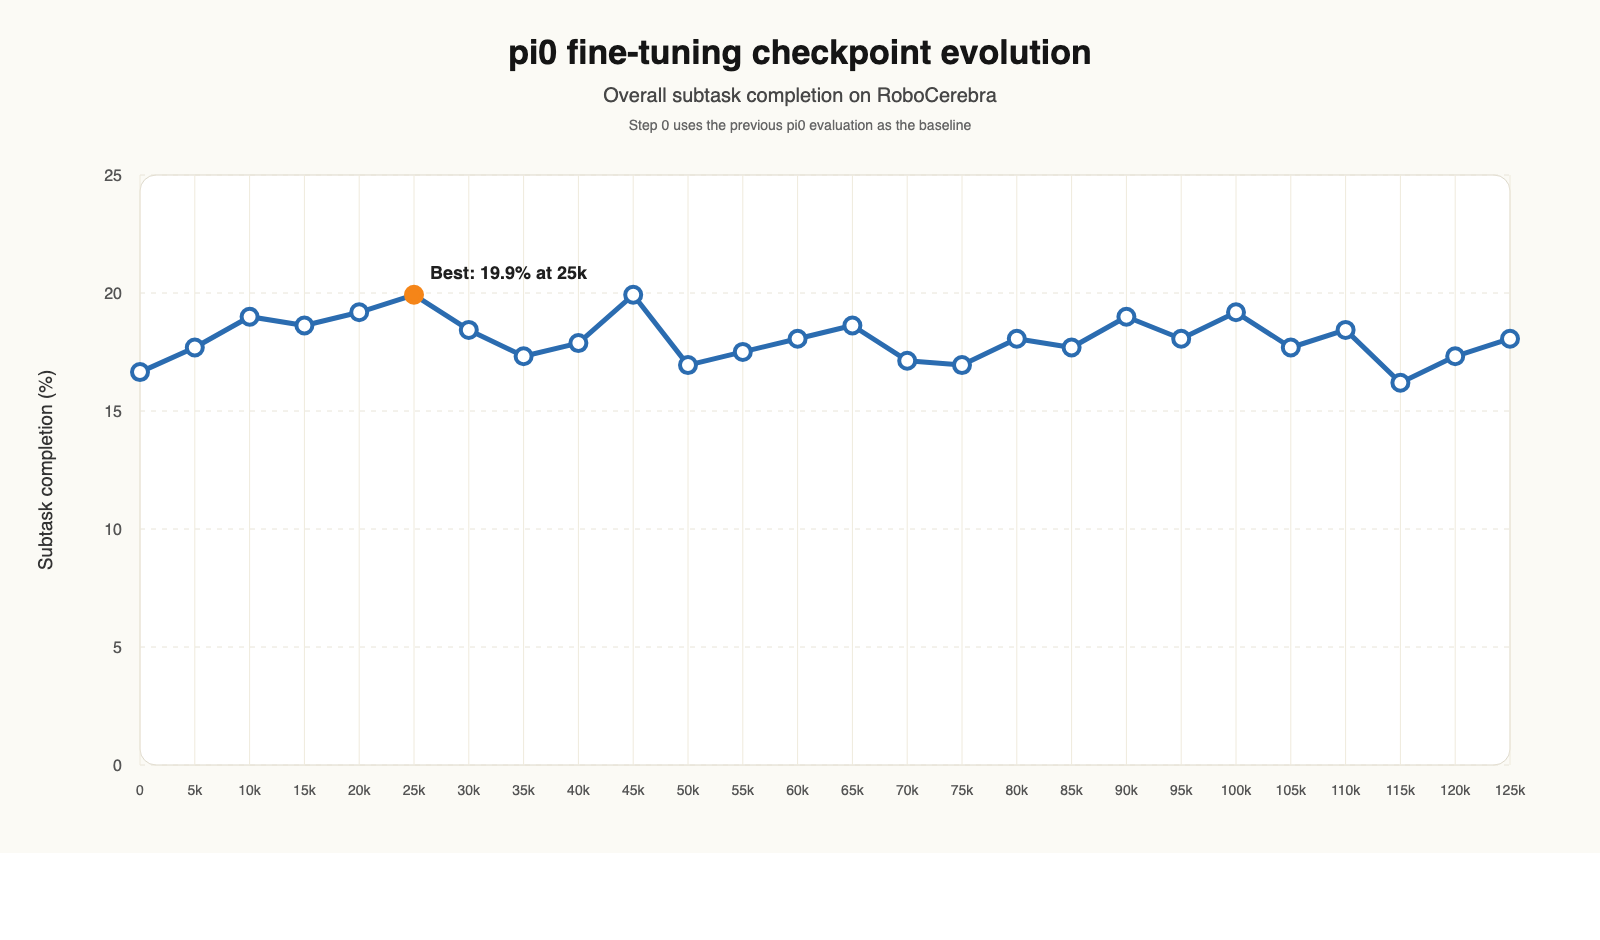
\includegraphics[width=0.92\linewidth]{pi0_checkpoint_progress_overall.png}
  \caption{Example local checkpoint plot: overall subtask completion is tracked separately from whole-episode success.}
\end{figure}

\section{Implementation Hooks in the Current Evaluator}

The proposed changes do not require replacing the evaluator. They can be added around the existing step parsing, resume, segment transition, and logging logic.

\begin{table}[htbp]
\centering
\caption{Existing evaluator components that can support the proposed subtask-failure logging.}
\begin{tabularx}{\linewidth}{>{\raggedright\arraybackslash}p{0.42\linewidth}Y}
\toprule
\textbf{Current component} & \textbf{How it supports the plan} \\
\midrule
\code{load_actions_with_steps} & Loads each goal predicate and its \code{task_step}, which is the key mapping from predicate success to subtask index. \\
\code{create_step_based_resume_handler} & Builds the set of subtasks that should already be complete before a resumed step. \\
\code{update_completion_tracking} & Already measures incremental subtask progress; this is the natural place to add missing-predicate and regression labels. \\
\code{handle_segment_transition} & Already switches between subtasks and can trigger GT-state restart after a detected failure. \\
\code{save_results_log} & Can be extended with a per-subtask attempt table while keeping the current aggregate success and subtask-rate metrics. \\
\bottomrule
\end{tabularx}
\end{table}

\section{Immediate Deliverables}

\begin{itemize}
  \item Patch the evaluator logs to emit one record per subtask attempt.
  \item Add flags for GT-state restart and robot-to-GT-pose recovery.
  \item Create three plots for the next report: first-failure histogram, recovery comparison, and chained-vs-isolated performance gap.
  \item Use these plots to decide whether future training should target planning, execution, or recovery behavior.
\end{itemize}

\begin{summarybox}
\textbf{Takeaway.}
RoboCerebra can be used as a diagnostic benchmark, not only a final-score benchmark. The benchmark can identify the failed subtask by comparing predicate progress at step boundaries, then test two recovery conditions: restart from the GT boundary after the previous subtask, or ask the robot to move back to the GT pose and continue.
\end{summarybox}

\end{document}
